\documentclass{standalone}
\usepackage{graphicx}	
\usepackage{amssymb, amsmath}
\usepackage{color}

\usepackage{tikz}
\usetikzlibrary{intersections, backgrounds}
\usepackage{pgfmath}

\definecolor{light}{RGB}{220, 188, 188}
\definecolor{mid}{RGB}{185, 124, 124}
\definecolor{dark}{RGB}{143, 39, 39}
\definecolor{highlight}{RGB}{180, 31, 180}
\definecolor{gray10}{gray}{0.1}
\definecolor{gray20}{gray}{0.2}
\definecolor{gray30}{gray}{0.3}
\definecolor{gray40}{gray}{0.4}
\definecolor{gray60}{gray}{0.6}
\definecolor{gray70}{gray}{0.7}
\definecolor{gray80}{gray}{0.8}
\definecolor{gray90}{gray}{0.9}
\definecolor{gray95}{gray}{0.95}

\begin{document}

\begin{tikzpicture}[scale=0.2, thick]

\fill[color=dark] (4, 1.5) circle (1);
\filldraw[fill=white, draw=dark] (0, 0) rectangle +(4, 3);

\draw[->, >=stealth, color=mid, line width=1] (-2, 1.5) -- (0, 1.5);
\node[right] at (-10.5, 1.5) { $h_{n} = n\,\mathrm{m}$ };

\draw[-, color=mid, dashed, line width=1] (2, 4) -- +(0, 5);

\fill[color=dark] (4, 1.5 + 10) circle (1);
\filldraw[fill=white, draw=dark] (0, 10) rectangle +(4, 3);

\draw[->, >=stealth, color=mid, line width=1] (-2, 11.5) -- (0, 11.5);
\node[right] at (-10.5, 11.5) { $h_{2} = 2\,\mathrm{m}$ };

\fill[color=dark] (4, 1.5 + 20) circle (1);
\filldraw[fill=white, draw=dark] (0, 20) rectangle +(4, 3);

\draw[->, >=stealth, color=mid, line width=1] (-2, 21.5) -- (0, 21.5);
\node[right] at (-10.5, 21.5) { $h_{1} = 1\,\mathrm{m}$ };

\fill[color=dark] (4, 31.5) circle (1);
\filldraw[fill=white, draw=dark] (0, 30) rectangle +(4, 3);

\draw[->, >=stealth, color=mid, line width=1] (-2, 31.5) -- (0, 31.5);
\node[right] at (-10.5, 31.5) { $h_{0} = 0\,\mathrm{m}$ };

\fill[color=mid] (12.5, 31.5) circle (2.1);
\node at (12.53, 31.8) {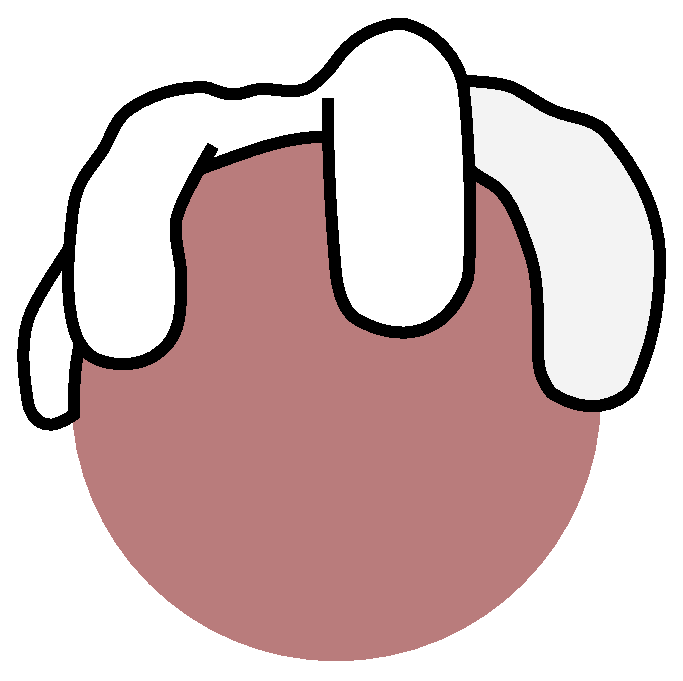
\includegraphics[width=1cm]{hands/closed_hand.eps}};

\draw[->, >=stealth, color=light, dashed, line width=1] (5.5, 31.5) -- +(12.5, 0);
\node[right] at (18, 31.5) { $t = 0$ };

\end{tikzpicture}

\end{document}  